\documentclass[12pt,final,twoside]{report}
%%%%%%%%%%%%%%%%%%%%%%%%%%%%%%%%%%%%%%%%%%%%%%%%%%%%%%%%%%%%%
% Some credits:
% The template initially was created by Prof. Dr. Holger Karl/Uni Paderborn '2006
% and was expanded and updated by Dipl.-Inform. Stefan Heinrich/Uni Paderborn/Uni Hamburg since 2008.
% Suggestions for changes are always welcome.
%%%%%%%%%%%%%%%%%%%%%%%%%%%%%%%%%%%%%%%%%%%%%%%%%%%%%%%%%%%%%
% Meta information:
\newcommand{\trtitle}{Visual-Audio Integration for Object Recognition}
\newcommand{\trtype}{Master thesis} %{Diplomarbeit} %{Dissertation}
\newcommand{\trcourseofstudies}{Intelligent Adaptive Systems} %{Bioinformatik} 
\newcommand{\trauthor}{Weipeng He}
\newcommand{\trauthortitle}{} %{Dipl.-Inform.\ }
\newcommand{\tremail}{2he@informatik.uni-hamburg.de}
\newcommand{\trmatrikelnummer}{6411529}
\newcommand{\trstrasse}{Hagenbeckstra\ss e 60}
\newcommand{\trort}{22527 Hamburg}
\newcommand{\trgutachterA}{\href{mailto:zhang@informatik.uni-hamburg.de}{Prof. Dr. Jianwei Zhang}}
\newcommand{\trgutachterB}{\href{mailto:maeder@informatik.uni-hamburg.de}{Dr. Andreas M\"ader}}
%\newcommand{\trbetreuung}{\href{mailto:tbd@informatik.uni-hamburg.de}{Dipl.-Inform. To Be Defined}}
\newcommand{\trfach}{Technical Aspects of Multimodal Systems, TAMS}
\newcommand{\trdate}{30.03.2015}
\newcommand{\trkeywords}{Multimodal, HMM, Object Recognition}

%%%%%%%%%%%%%%%%%%%%%%%%%%%%%%%%%%%%%%%%%%%%%%%%%%%%%%%%%%%%%
% Languages:

% Falls die Ausarbeitung in Deutsch erfolgt:
% \usepackage[german]{babel}
% \usepackage[T1]{fontenc}
% \usepackage[latin1]{inputenc}
% \usepackage[latin9]{inputenc}                     
% \selectlanguage{german}

% If the thesis is written in English:
\usepackage[english]{babel}                         
\selectlanguage{english}

%%%%%%%%%%%%%%%%%%%%%%%%%%%%%%%%%%%%%%%%%%%%%%%%%%%%%%%%%%%%%
% Bind packages:
\usepackage{acronym}                    % Acronyms
\usepackage{algorithmic}                % Algorithms and Pseudocode
\usepackage{algorithm}                  % Algorithms and Pseudocode
\usepackage{amsfonts}                   % AMS Math Packet (Fonts)
\usepackage{amsmath}                    % AMS Math Packet
\usepackage{amssymb}                    % Additional mathematical symbols
\usepackage{amsthm}
\usepackage{booktabs}                   % Nicer tables
%\usepackage[font=small,labelfont=bf]{caption} % Numbered captions for figures
\usepackage{color}                      % Enables defining of colours via \definecolor
\definecolor{uhhRed}{RGB}{226,0,26}     % Official Uni Hamburg Red
\definecolor{uhhGrey}{RGB}{136,136,136} % Official Uni Hamburg Grey
\definecolor{uhhLightGrey}{RGB}{220, 220, 220}
\usepackage{fancybox}                   % Put equations in a frame
\usepackage{fancyhdr}                   % Packet for nicer headers
%\usepackage{fancyheadings}             % Nicer numbering of headlines
\usepackage[body={5.8in,9in}]{geometry} % Type area (size, margins...)

%\geometry{a4paper,outer=3.35cm}        % !!!Release version (Normal margins)
%\geometry{a4paper,outer=2.5cm}         % !!!Print version (Additional margin on the left for the binding)
%\geometry{a4paper}                     % !!!Proofread version (Additional margin on the right for corrections)
\geometry{a4paper,outer=3.15cm}         % !!!Draft version (Same margins on left and right)
%\geometry{paperheight=10.0in,paperwidth=6.4in,top=0.51in,left=0.3in}  % !!!Developer version (Minimal margins)

\usepackage{graphicx}                   % Inclusion of graphics
%\usepackage{latexsym}                  % Special symbols
\usepackage{longtable}                  % Allow tables over several parges
\usepackage{listings}                   % Nicer source code listings
\usepackage{multicol}                   % Content of a table over several columns
\usepackage{multirow}                   % Content of a table over several rows
\usepackage{rotating}                   % Alows to rotate text and objects
\usepackage{tabularx}                   % Tables with fixed width but variable rows
\usepackage{url,xspace,boxedminipage}   % Accurate display of URLs

\usepackage{subcaption}

%%%%%%%%%%%%%%%%%%%%%%%%%%%%%%%%%%%%%%%%%%%%%%%%%%%%%%%%%%%%%
% PDF Information und Definitions:
\author{\trauthor}

\ifx\pdftexversion\undefined
\usepackage{hyperref}
\else
\usepackage[colorlinks=false,           % link is colores (true) or has colored frame (false)
            linkcolor=uhhRed,           % case colorlinks=true: define color.
            urlcolor=uhhRed,
            citecolor=uhhRed,
            bookmarks,                  % Place bookmarks erstellen
            bookmarksopen=true,         % Bookmarks will be shown at start (true/false)
            pdfpagemode=UseOutlines,    
            bookmarksopenlevel=1,       % Define the depth of shown links
            bookmarksnumbered,          % Numbers of chapers in Bookmarks
            pdftitle={\trtitle},
            pdfsubject={\trtype},
            pdfkeywords={\trkeywords},
            pdfauthor={\trauthor},
            plainpages=false
            ]{hyperref}
\fi

\ifx\pdftexversion\undefined
\else
\pdfoutput=1                            % Disable PDF-Output
\pdfimageresolution=1200
\pdfcompresslevel=2                     % 0 = no compression, 9 = strongest compression
\fi

%%%%%%%%%%%%%%%%%%%%%%%%%%%%%%%%%%%%%%%%%%%%%%%%%%%%%%%%%%%%%
% Configurationen:

\hyphenation{whe-ther}                  % Manually use: "\-" in a word: Staats\-ver\-trag

%\lstloadlanguages{C}                   % Set the default language for listings
\DeclareGraphicsExtensions{.pdf,.svg,.jpg,.png,.eps} % first try pdf, then eps, png and jpg
\graphicspath{{./fig/}}                 % Path to a folder where all pictures are located
\pagestyle{fancy}                       % Use nicer header and footer

% Redefine the environments for floating objects:
\setcounter{topnumber}{3}
\setcounter{bottomnumber}{2}
\setcounter{totalnumber}{4}
\renewcommand{\topfraction}{0.9}        %Standard: 0.7
\renewcommand{\bottomfraction}{0.5}     %Standard: 0.3
\renewcommand{\textfraction}{0.1}       %Standard: 0.2
\renewcommand{\floatpagefraction}{0.8}  %Standard: 0.5

% Tables with a nicer padding:
\renewcommand{\arraystretch}{1.2}

% Chapter and Sections will not be written in capitals
\renewcommand{\chaptermark}[1]{\markboth{\chaptername \ \thechapter.\ #1}{}}
\renewcommand{\sectionmark}[1]{\markright{\thesection.\ #1}}

%%%%%%%%%%%%%%%%%%%%%%%%%%%%
% Additional 'theorem' and 'definition' blocks:
\theoremstyle{plain}
\newtheorem{theorem}{Theorem}[chapter]
%\newtheorem{theorem}{Satz}[chapter]    % Wenn in Deutsch geschrieben wird.
\newtheorem{axiom}{Axiom}[chapter]     
%\newtheorem{axiom}{Fakt}[chapter]      % Wenn in Deutsch geschrieben wird.
%Usage:%\begin{axiom}[optional description]%Main part%\end{fakt}

\theoremstyle{definition}
\newtheorem{definition}{Definition}[chapter]

%Additional types of axioms:
\newtheorem{lemma}[axiom]{Lemma}
\newtheorem{observation}[axiom]{Observation}

%Additional types of definitions:
\theoremstyle{remark}
%\newtheorem{remark}[definition]{Bemerkung} % Wenn in Deutsch geschrieben wird.
\newtheorem{remark}[definition]{Remark} 

%%%%%%%%%%%%%%%%%%%%%%%%%%%%
% Provides TODOs within the margin:
\newcommand{\TODO}[1]{\marginpar{\emph{\small{{\bf TODO: } #1}}}}

%%%%%%%%%%%%%%%%%%%%%%%%%%%%
% Abbreviations and mathematical symbols
\newcommand{\modd}{\text{ mod }}
\newcommand{\RS}{\mathbb{R}}
\newcommand{\NS}{\mathbb{N}}
\newcommand{\ZS}{\mathbb{Z}}
\newcommand{\dnormal}{\mathit{N}}
\newcommand{\duniform}{\mathit{U}}

\newcommand{\erdos}{Erd\H{o}s}
\newcommand{\renyi}{-R\'{e}nyi}
% it is recommented to define complex terms as expression/newcommand and use the expression in the tex instead.

%%%%%%%%%%%%%%%%%%%%%%%%%%%%%%%%%%%%%%%%%%%%%%%%%%%%%%%%%%%%%
% Document:

\begin{document}

\pagenumbering{Roman}                   % Roman pagenumbering for lists and meta pages
\renewcommand{\headheight}{14.5pt}      % Size of headings

\thispagestyle{empty}
\fancyhead[LO,RE]{}                     % Define the header style for the meta pages

%%%%%%%%%%%%%%%%%%%%%%%%%%%%
% Cover sheet

\begin{titlepage}
%---Possibility 1:
    \begin{flushleft}
        
\includegraphics[width=85mm]{uhhLogoL.pdf}\\
    \end{flushleft}
%---Possibility 2:
%\includegraphics*[width=0.09\textwidth]{uhhIconR_}
%\parbox[c]{10cm}{
%    \begin{center}
%    Universit�t Hamburg --- MIN-Fakult�t\\
%    \trfachgruppe
%    \end{center}
%    }\hfill
%\includegraphics*[width=0.09\textwidth]{infIcon_}
%\vspace{0.2cm}
%---
    \rule{\textwidth}{0.4pt}
        \newline
        \vspace{2.0cm}
        \begin{center}
          \LARGE \textbf{\trtitle}
        \end{center}
    \vspace{2.0cm}
    \begin{center}
      \textbf{\trtype}\\
      %am Fachgebiet \trfach\\
      im Arbeitsbereich \trfach\\
      \trgutachterA\medskip\\
      Department Informatik\\
      MIN-Fakult\"at\\
      Universit\"at Hamburg \\[0.5cm]
      vorgelegt von \\
      \textbf{\trauthortitle\href{mailto:\tremail}{\trauthor}}\\
      am\\
      \trdate
    \end{center}
    \vspace{1cm}
    \begin{center}
    \begin{tabular}{ll}
    Gutachter: & \trgutachterA \\
                   & \trgutachterB \\
    %Betreuung: & \trbetreuung \\    	% Adviser are not allowed to demand getting credited, but are happy getting credited by the students initiative
    \end{tabular}
    \end{center}
    \vfill
    \begin{tabular}{l}
    \trauthor \\
    Matrikelnummer:  \trmatrikelnummer \\
    \trstrasse \\
    \trort
    \end{tabular}
    \newline
    \rule{\textwidth}{0.4pt}
    \newpage 
\end{titlepage}

    %backsite of cover sheet is empty!
\thispagestyle{empty}
\hspace{1cm}
\newpage

%%%%%%%%%%%%%%%%%%%%%%%%%%%%
% Abstract:
\section*{Abstract}\label{sec:abstract}
%\fancyhead[LE,RO]{\it Abstract}
%\addcontentsline{toc}{chapter}{\numberline{}Abstract}
Your English abstract here (mandatory if written in English and recommended otherwise).

\fancyhead[LE,RO]{\it Abstract}

\cleardoublepage

%%%%%%%%%%%%%%%%%%%%%%%%%%%%
% Lists:
%\setcounter{tocdepth}{1}               % depth of the table of contents (for BSc and MSc Thesis 1 is recommented)
\fancyhead[LE,RO]{\it Contents}
\tableofcontents
\cleardoublepage
% List of Figures and List of tables are optional. -> Not needed in most theses.
\fancyhead[LE,RO]{\it List of Figures}
\listoffigures
\cleardoublepage
\fancyhead[LE,RO]{\it List of Tables}
\listoftables
\cleardoublepage
%\lstlistoflistings
%\cleardoublepage

\fancyhead[LE]{\it \leftmark}           % Define the header style for the text pages
\fancyhead[RO]{\it \rightmark}          % Define the header style for the text pages
\fancyhead[LO,RE]{}                     % Define the header style for the text pages

%%%%%%%%%%%%%%%%%%%%%%%%%%%%
% The content will be included here:
\pagenumbering{arabic}

\chapter{Introduction}\label{introduction}

\section{Motivation}

\section{Related Work}

\section{Contribution}

\section{Thesis Outline}


\cleardoublepage

\chapter{Background}\label{background}

In this chapter, three related fields regarding visual-audio object recognition will be reviewed. First, the traditional methods of object recognition based on visual information exclusively will be introduced. Then, the state-of-the-art in multimodal object recognition will be presented. Finally, the application of visual-audio integration in speech recognition will be explained.

\section{Visual Object Recognition}
Visual object recognition has been extensively studied in the recent decade. Vision is very essential for both humans and artificial agents to recognize an object, since it provides the most direct and informational clue about the object. Numerous methods have been proposed for visual object recognition and they have been used in a variety of applications.

\begin{figure}[tbhp]
  \centering
  \begin{subfigure}[b]{.3\textwidth}
    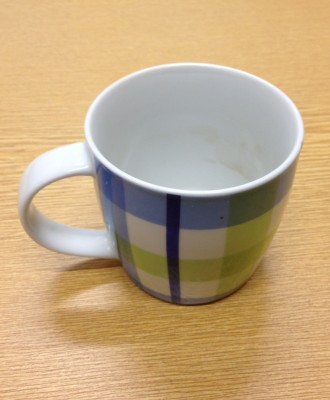
\includegraphics[width=\textwidth]{themug}
    \caption{Sam's coffee mug}
  \end{subfigure}
  ~
  \begin{subfigure}[b]{.3\textwidth}
    \centering
    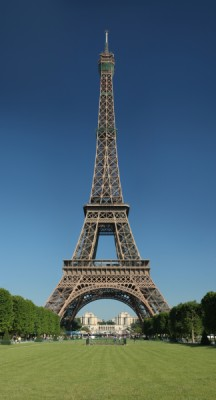
\includegraphics[width=.7\textwidth]{tour_eiffel}
    \caption{The Eiffel Tower\footnotemark}
  \end{subfigure}
  ~
  \begin{subfigure}[b]{.3\textwidth}
    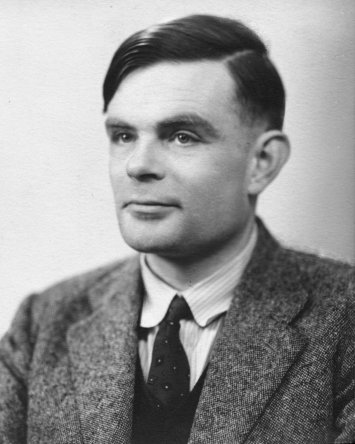
\includegraphics[width=\textwidth]{turing}
    \caption{Alan Turing}
  \end{subfigure}
  \caption{Examples of specific objects.}
  \label{fig:specific}
\end{figure}
\footnotetext{``Eiffel Tower'' by \href{http://commons.wikimedia.org/wiki/User:Benh}{Benh}. Licensed under \href{http://creativecommons.org/licenses/by-sa/3.0}{CC BY-SA 3.0}.}

Concerning object recognition, there are two types of tasks been studied: specific object recognition and object category recognition \cite{grauman_visual_2011}. The specific object recognition is the task of recognizing a particular object, place or person. Examples of this case are Sam's coffee mug, the Eiffel tower or Alan Turing as shown in Figure~\ref{fig:specific}. These objects (or person) have little variation in appearance and shape. 

\begin{figure}[tbhp]
  \centering
  \begin{subfigure}[b]{.45\textwidth}
    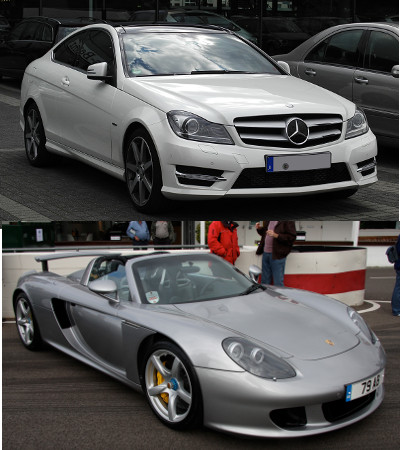
\includegraphics[width=.89\textwidth]{cars} % figure from public domain
    \caption{Cars\footnotemark}
  \end{subfigure}
  ~
  \begin{subfigure}[b]{.45\textwidth}
    \centering
    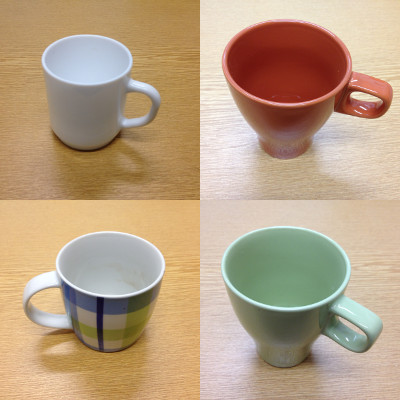
\includegraphics[width=\textwidth]{mugs}
    \caption{Coffee Mugs}
  \end{subfigure}
  \caption{Examples of generic objects categories.}
  \label{fig:generic}
\end{figure}
\footnotetext{The upper photo is ``Mercedes-Benz C 250'' by \href{http://commons.wikimedia.org/wiki/User:M_93}{M 93}. Licensed under \href{http://creativecommons.org/licenses/by-sa/3.0/de}{CC BY-SA 3.0 de}.
The lower photo is ``Porsche Carrera GT'' by \href{http://www.flickr.com/people/32659528@N00}{Brian Snelson}. Licensed under \href{http://creativecommons.org/licenses/by/2.0}{CC BY 2.0}}

Unlike the specific case, generic object category recognition cope with classifying an instance to a category, for example, telling a object is an instance of cars or coffee mugs (see Figure~\ref{fig:generic}). In this case, the objects belongs to the same category have the same conceptual meaning, but may vary in appearance and shape. A category can also be a function or an attribute of the object, like objects that can be sit on or soft objects.

As we have seen, these two types of tasks try to solve different problems. Therefore, different features and learning methods are required. Some of the approaches will be discussed in the rest of this section.

\subsection{Visual Specific Object Recognition}
One of the approaches which have achieved robust and efficient result in specific object recognition is proposed by Lowe \cite{lowe_object_1999}. His approach first extracts SIFT features from the image. Scale Invariant Feature Transform (SIFT)is a kind of local feature that is invariant to image translation, scaling, and rotation. Then, the extracted features are matched between train and test images. In the final step, the matched features are verified to confirm they are in a consistent geometric configuration. This approach has been widely used in robotic visual systems \cite{grauman_visual_2011}.

\subsection{Visual Object Category Recognition}
While specific object recognition can be solved as matching of local features, the task of object category recognition requires representations that capture the common characteristics of different instances in the same class. Example systems for object category recognition include the Viola-Jones face detector \cite{viola_rapid_2001}, bag-of-words model \cite{csurka_visual_2004} and HOG person detector \cite{dalal_histograms_2005}. 

The bag-of-words model \cite{csurka_visual_2004} for object category recognition is motivated by the bag-of-words model in text categorization. The visual image with a collection of local feature descriptors is analog to a document with a collection of words. In practice, a vocabulary of visual words is first constructed with clustering the feature descriptors from a number of images. Here, descriptors like SIFT or SURF can be used. Then, an image can be represented as a histogram of the vocabulary. After that, classifiers like support vector machine or Na\"ive Bayes can be used for categorization. This bag-of-words model achieved high and robust categorization accuracy.

Sivic et al. \cite{sivic_discovering_2005} used the bag-of-words model for unsupervised object categorization. Same as \cite{csurka_visual_2004}, given a collection of images, the feature of the images is first extracted as a bag of visual words. Then, generative models like Latent Semantic Analysis (pLSA) and Latent Dirichlet Allocation (LDA) are learned from the representation vectors. These models, which are successfully used for text analysis finding document topics, can also be used for finding the underlying common features of an object category. Since their learning method is unsupervised, it is applicable to a large unlabeled image set.

\section{Multimodal Object Recognition}
When thinking of how humans recognize objects, we use not only visual information, but also perceptions of other modalities, like auditory, haptic and olfactory perception. These extra perceptions provide complementary information. For example, a paper cup might have the same shape as a ceramic cup, and it is difficult to distinguish them only with vision. However, if we make some sound of them by knocking or touch them, we can use auditory or haptic information to tell the difference. This idea of multimodal object recognition is also applied to robotic systems.

\subsection{Multimodal pLSA Model}
Nakamura et al. \cite{nakamura_multimodal_2007} proposed an unsupervised object categorization method for robots based on visual, audio and haptic information. They used a multimodal pLSA model, which is extended from the pLSA model described in \cite{sivic_discovering_2005}, for the categorization.

In their experiment, a robot hand was used to grasp and shake the objects. During the interaction, visual, audio and haptic information were collected by a camera at the side, a microphone and pressure sensors on the robot finger. Afterwards, the data were processes separately as follows:
\begin{description}
  \item[Visual Information] \hfill \\
    Each image frame was represented using a bag-of-words model with scale and affine invariant salient region detector \cite{mikolajczyk_scale_2004} and SIFT descriptor \cite{lowe_distinctive_2004}. The visual vocabulary was generated by clustering the local descriptors in a collection of images into 600 clusters using k-means algorithm. The collection of images are 100 indoor images, which are independent of the objects in their experiment.
  \item[Audio Information] \hfill \\
    For each audio frame, a 13-dimensional MFCC feature was first calculated and then represented as a bag-of-words model with a vocabulary of 50 clusters. The vocabulary was generated with speech and noises.
  \item[Haptic Information] \hfill \\
    For each grasp of an object, a 2-dimensional feature vector was collected by the pressure sensors on the robot finger. Then, the feature vectors were vector quantized with 5 clusters, which was generated in advance.
\end{description}

They tested the unsupervised categorization on 40 objects in 8 categories. The objects were toys like stuffed toys, rattles, tambourines and balls. It was shown that their categorization result of using three modalities was identical to the categorization result of human subject. However, categorization using one modality alone did not work as well.

Furthermore, they also tested the performance of category and property inference of an unseen object. By using ``fold in'' heuristic \cite{hofmann_probabilistic_1999}, they correctly inferred the categories of all the objects in leave-one-out cross validation. For the property inference, their method can infer the auditory and haptic properties when given only the visual cue of the object.

\subsection{Behavior-Grounded Relational Learning}
Another multimodal object categorization approach is the behavior-grounded relational learning proposed by Sinapov and Stoytchev \cite{sinapov_object_2011}. Different from the aforementioned multimodal pLSA approach, they used different features and a supervised learning method.

They used an upper-torso humanoid robot to interact with the objects and collect proprioceptive and auditory information. The interactions included five exploratory behaviors, which are lift, shake, drop, crush and push. The proprioceptive data was recorded with 7 joint torque sensors and the auditory data was recorded by a microphone mounted on the robot head.

The method for extracting proprioceptive and auditory features were described in \cite{bergquist_interactive_2009} and \cite{sinapov_interactive_2009}, respectively. Since the interactions spanned over time, the data recorded were sequences of vectors. Here, a proprioceptive vector consisted of the joint torques, and a auditory vector was a Short Time Fourier Transform (STFT) of the raw audio recording. These vectors were further quantized using Self-organizing Map (SOM). Then, one modality of one behavior execution could be represented as a sequence of nominal values, that are the states in the SOM. Furthermore, the similarity between two different sequence can be calculated with Needleman-Wunch alignment algorithm \cite{needleman_general_1970}.

Based on the similarity of executions recordings, they constructed the relational features. The relational features of an object are the average similarities to a known object sets (for example the objects which are or are not plastic cups). The sets were the objects of the 6 categories, which are plastic cups, pop cans, metal objects, soft objects, empty bottles and objects with content. And, with 10 sensorimotor context (a behavior-modality combination), a object is represented by a $10 \times 2 \times 6 = 120$ dimensional vector.

Consequently, they applied discriminative methods, like Support Vector Machine, k-Nearest Neighbor and Decision Tree, for learning the object category. They evaluated these methods with Cohen's kappa coefficient \cite{cohen_coefficient_1960}. Their approach achieved kappa coefficient from 0.4 to .85 for the recognition.

\section{Visual-Audio Speech Recognition}


\cleardoublepage

\chapter{Approach}\label{approach}

\cleardoublepage

\chapter{Results}\label{results}

\cleardoublepage

\chapter{Conclusion}\label{conclusion}


\cleardoublepage

%%%%%%%%%%%%%%%%%%%%%%%%%%%%
% Appendices:
% these are optional! For most Bachelor-theses and some Master-thesis none of them is needed. 
% Just comment them if not needed.
\appendix
\fancyhead[LO,RE]{}                      % Define the header style for the appendixpages

\fancyhead[LE,RO]{\it Anhang A. Nomenclature}                %Adapt letter!
\chapter{TBD}\label{app:nomenclature}

\cleardoublepage

% ... add as much appendices as you need (one can also add source code, for example)

%\fancyhead[LE]{\it \leftmark}
%\chapter{}
\fancyhead[LE,RO]{\it Bibliography}       % A bibliography never have a letter or numbering!
    \bibliographystyle{plain}             % Style for presenting the literature
    \addcontentsline{toc}{chapter}{Bibliography}% Add to the TOC
    \bibliography{thesis}
\cleardoublepage

%%%%%%%%%%%%%%%%%%%%%%%%%%%%
% Formal page 1
\vspace{2cm}
\chapter*{Erkl\"arung der Urheberschaft}
\fancyhead[LE]{\it Erkl�rung der Urheberschaft}
Ich versichere an Eides statt, dass ich die \trtype{} im Studiengang \trcourseofstudies{} selbstst\"andig verfasst und keine anderen als die angegebenen Hilfsmittel -- insbesondere keine im Quellenverzeichnis nicht benannten Internet-Quellen -- benutzt habe. Alle Stellen, die w\"ortlich oder sinngem\"a{\ss} aus Ver\"offentlichungen entnommen wurden, sind als solche kenntlich gemacht. Ich versichere weiterhin, dass ich die Arbeit vorher nicht in einem anderen Pr�fungsverfahren eingereicht habe und die eingereichte schriftliche Fassung der auf dem elektronischen Speichermedium entspricht.

%Ich versichere an Eides statt, dass ich die vorliegende \trtype{} selbstst\"andig und ohne unerlaubte Hilfe Dritter angefertigt habe. Alle Stellen, die inhaltlich oder w\"ortlich aus anderen Ver\"offentlichungen stammen, sind kenntlich gemacht. Diese Arbeit lag in gleicher oder \"ahnlicher Weise noch keiner Pr\"ufungsbeh\"orde vor und wurde bisher noch nicht ver\"offentlicht.

\vspace{4cm}
\noindent Ort, Datum \hfill Unterschrift

%The backcover is always empty
\newpage
\thispagestyle{empty}
\hspace{1cm}
\newpage

%%%%%%%%%%%%%%%%%%%%%%%%%%%%
% Formal page 2
\vspace{2cm}
\chapter*{Erkl\"arung zur Ver\"offentlichung}
\fancyhead[LE]{\it Erkl�rung der Ver�ffentlichung}
Ich erkl\"are mein Einverst�ndnis mit der Einstellung dieser \trtype{} in den Bestand der Bibliothek.

\vspace{4cm}
\noindent Ort, Datum \hfill Unterschrift

%The backcover is always empty
\newpage
\thispagestyle{empty}
\hspace{1cm}
\newpage

\end{document}
%EOF

